\section{Tratamiento de grandes cantidades de datos}

Una de las caracter�sticas m�s significativas en el tratamiento de genoma, es la gran cantidad de datasets que se generan. Estos datos hay que manejarlos de forma eficiente y adecuada, para preservar su integridad y a la vez que su acceso sea lo m�s r�pido posible. Esta secci�n est� dedicada a distintos modelos que se utilizan hoy d�a para el tratamiento de una gran cantidad de datos.

\subsection{MapReduce}

MapReduce\cite{mapreducesimp} es un modelo de programaci�n con una implementaci�n asociada para procesar y generar grandes datasets. En los �ltimos a�os se han venido implementando cientos de c�digos de prop�sito especial (Google implement� la mayor�a) para procesar grandes cantidades de datos en bruto, c�mo documentos o peticiones web, para obtener distintos tipos de informaci�n derivada (�ndices, grafos de webs, res�menes...). La mayor�a de estos procesos son triviales y no requieren de un computo intensivo, pero los datos de entrada son demasiado grandes y tienen que ser distribuidos entre miles de m�quinas para procesarlos en un tiempo razonable.\\

Todo esto generaba cada vez m�s complejidad, por lo que la reacci�n fue el dise�o de un nuevo tipo de abstracci�n que permitiese realizar simples c�mputos ocultando detalles del paralelismo, la distribuci�n de los datos y la carga, ofreciendo adem�s tolerancia a fallos. Todo esto incluido en una simple librer�a, as� fue como naci� MapReduce (de mano de Google).\\

El computo en este modelo se basa en un conjunto de pares clave/valor de entrada, que generan un conjunto de pares clave/valor de salida. Esto se genera mediante dos funciones que el programador debe definir: \textit{Map} y \textit{Reduce}. \textit{Map} obtiene un par de entrada y genera un conjunto de pares intermedios. Estos pares intermedios son recopilados internamente por la librer�a y los agrupa por su clave intermedia, pas�ndolos seguidamente a la funci�n \textit{Reduce}. La funci�n \textit{Reduce} acepta una de las claves intermedias y el conjunto de valores para esa clave, combin�ndolos para generar el conjunto de valores de salida. La Figura \ref{fig:mapreduce} muestra gr�ficamente un ejemplo para contar palabras usando el modelo \textit{MapReduce}.\\


\begin{figure}
\centering
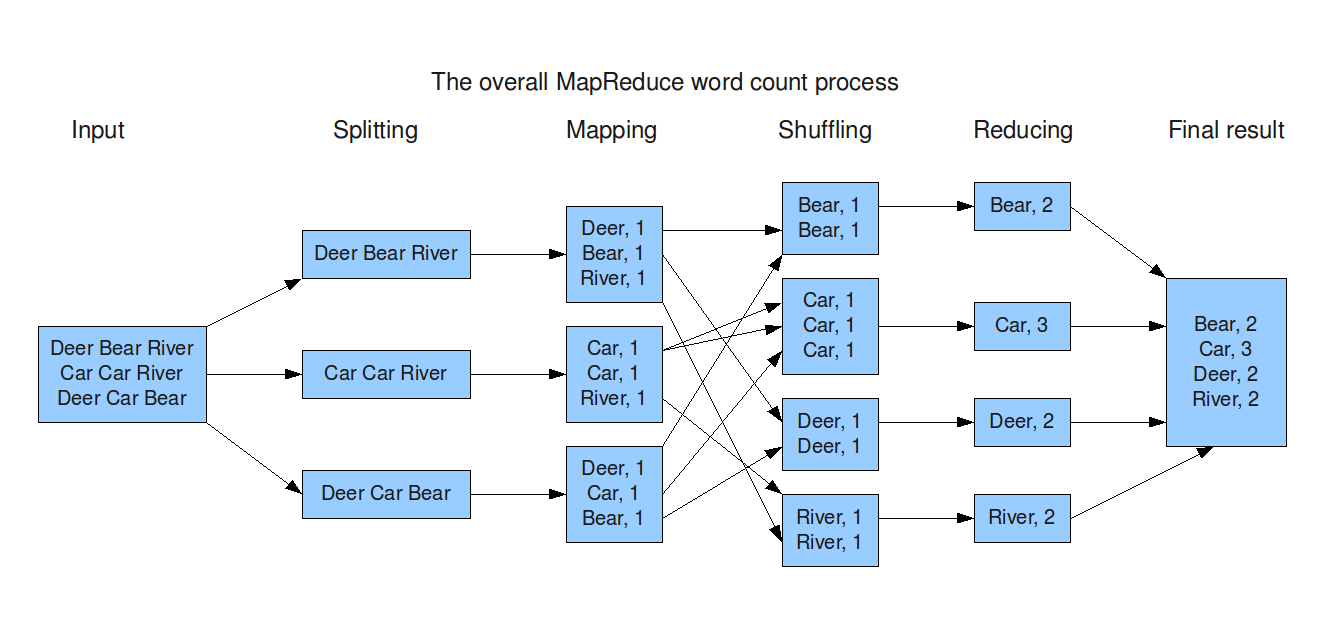
\includegraphics[width=0.8\textwidth]{mapreduce.png}
\caption{Modelo paralelo \textit{MapReduce} para contar palabras.\label{fig:mapreduce}}
\end{figure}